\newpage
\section{Otimização da torção da asa}\label{sec:torcao}

O diagnóstico da Seção~\ref{sec:secao_critica} para a asa sem torção, com
estol começando na ponta sobre o aileron, motivou uma realimentação de
projeto no espírito do Lab 03: escolher a torção geométrica das estações
da asa por otimização com restrição. O problema formulado foi

\begin{equation*}
    \min_{\theta}\; C_{D,\mathrm{ff}}(\theta)
    \quad \text{sujeito a} \quad
    \eta_{\mathrm{crit}}(\theta) \leq 0{,}50,
\end{equation*}

em que $\theta$ reúne as torções das estações $\eta = 0{,}398$, 0,56, 0,90
e 1,0, com a raiz fixa em zero como referência e limites de $-6^\circ$ a
$+3^\circ$. A função objetivo é o arrasto induzido no plano de Trefftz da
aeronave trimada no ponto de projeto ($M = 0{,}85$, $C_L = 0{,}5053$,
arfagem compensada pelo profundor). A restrição exige que a seção crítica
do estol em $M = 0{,}2$ fique na metade interna da asa, antes do aileron,
com folga de $0{,}5^\circ$ de ângulo de ataque sobre a região externa.

A estrutura do método de malha de vórtices foi explorada para resolver o
problema sem otimização cara. A distribuição de sustentação é linear nas
torções e no ângulo de ataque, de modo que o modelo do estol sai de duas
rodadas de base e uma por variável. O arrasto induzido é quadrático nas
torções, e o modelo exato da função objetivo sai de quinze rodadas no
ponto de projeto. Sobre esses modelos o problema foi resolvido por
programação sequencial quadrática com multipartida, e o ótimo foi
verificado com rodadas adicionais do AVL fora dos modelos.

\begin{table}[H]
\centering
\caption{Torção otimizada por estação e comparação antes e depois.}\label{tab:torcao}
\renewcommand{\arraystretch}{1.25}
\begin{tabular}{lc@{\hspace{2.5em}}lcc}
\toprule
Estação $\eta$ & Torção [graus] & Grandeza & Sem torção & Com torção \\
\midrule
0,000 & 0,00 & $C_{D,\mathrm{ff}}$ em cruzeiro & 0,01027 & 0,00957 \\
0,101 & 0,00 & $C_D$ no ponto de projeto (CG diant.) & 0,02829 & 0,02655 \\
0,398 & $+2{,}03$ & $C_{L\mathrm{max}}$ (CG diant.\ trimado) & 0,829 & 1,036 \\
0,560 & $-4{,}86$ & Estação crítica do estol $\eta$ & 0,89 & 0,45 \\
0,900 & $-5{,}19$ & $i_t$ de cruzeiro (CG diant.) [graus] & $-8{,}40$ & $-6{,}06$ \\
1,000 & $-6{,}00$ & $\alpha$ de estol [graus] & 11,0 & 14,7 \\
\bottomrule
\end{tabular}
\end{table}

\begin{figure}[H]
\centering
\caption{Distribuição de torção otimizada e o efeito sobre o estol: a
seção crítica migra da ponta ($\eta = 0{,}89$) para a metade interna da
asa ($\eta = 0{,}45$).}\label{fig:torcao}
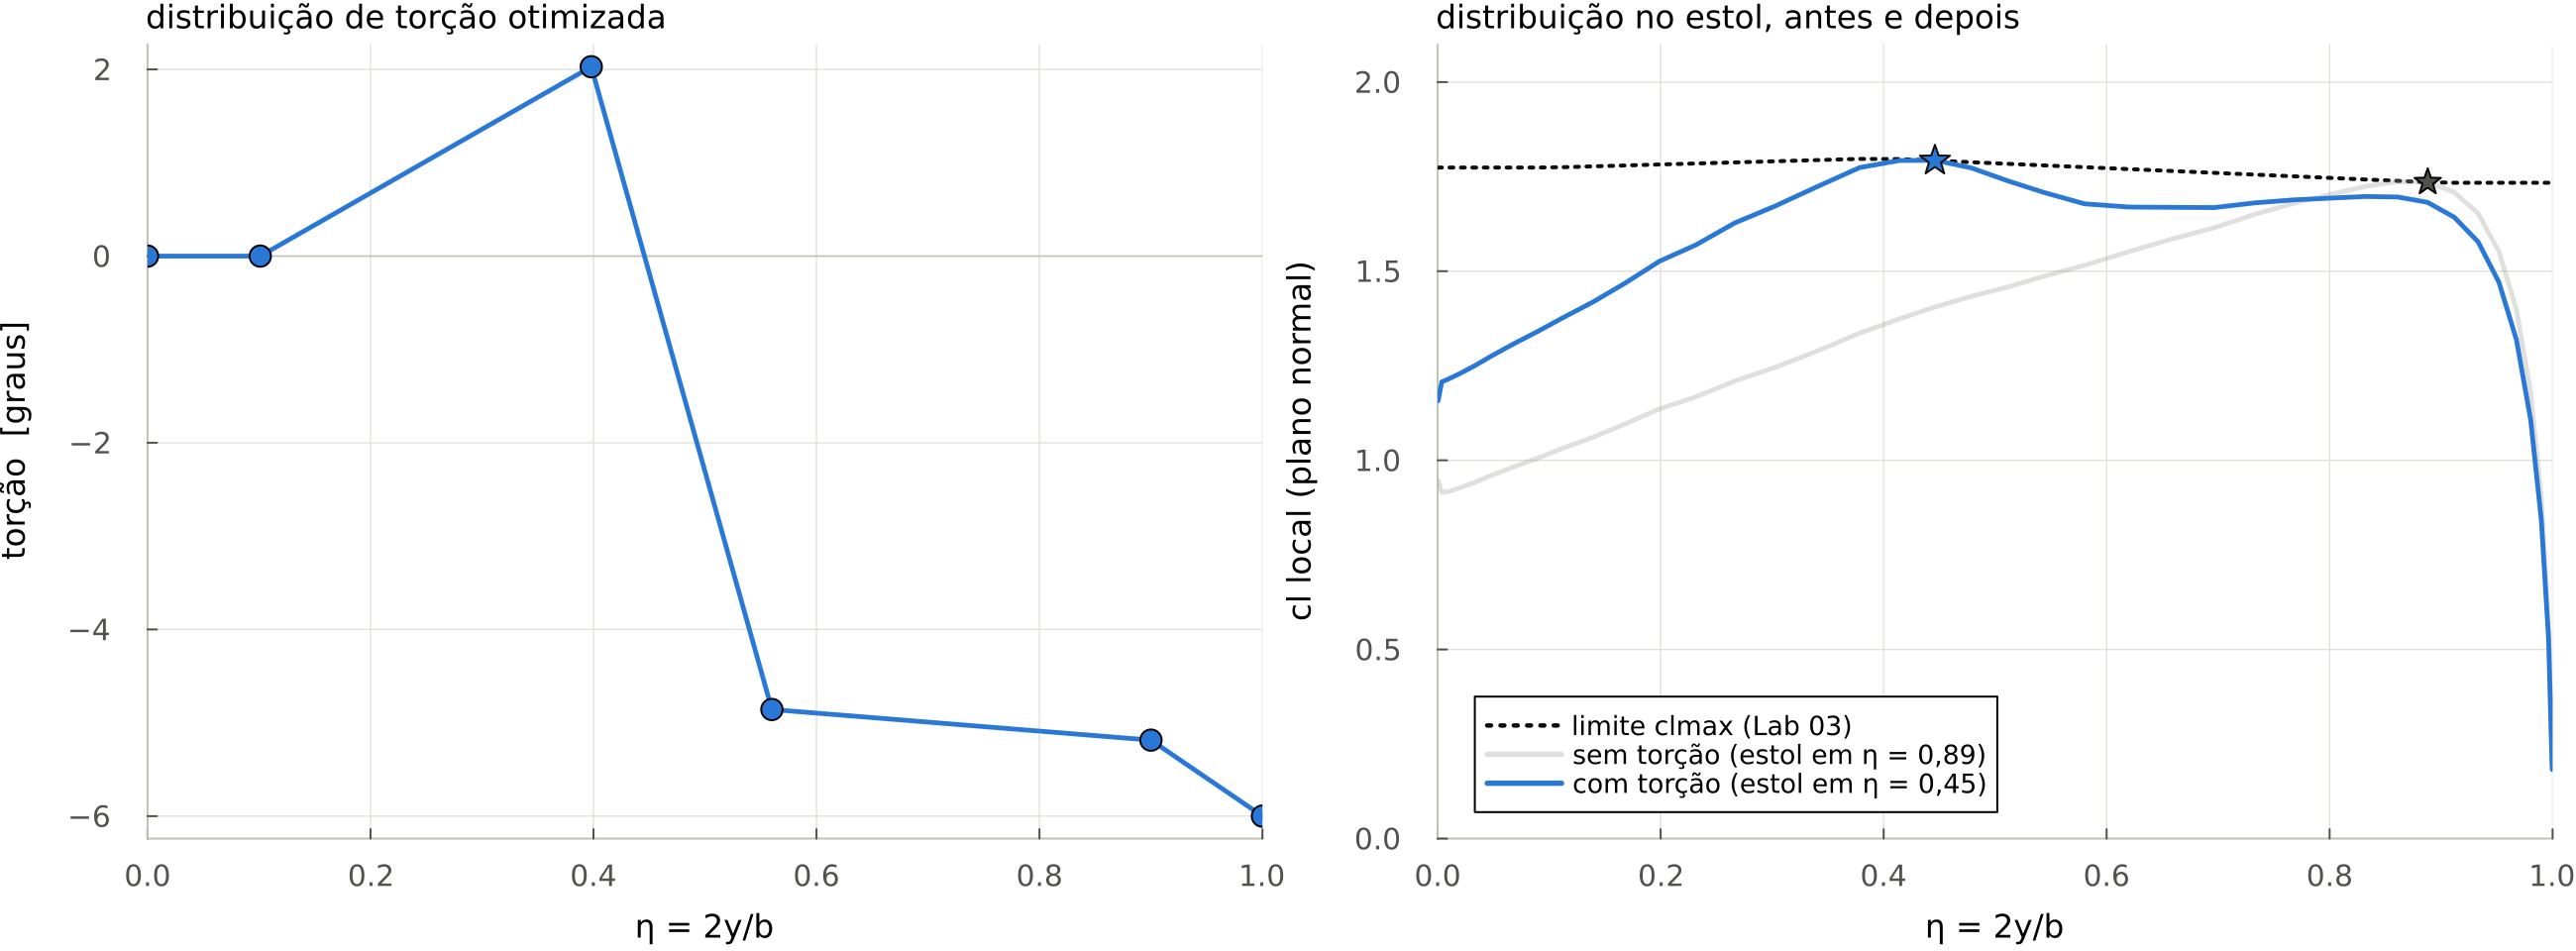
\includegraphics[width=\linewidth]{images/06_torcao/torcao_antes_depois.png}
\end{figure}

O resultado mais importante é que a torção não custou arrasto: o washout
reduziu o arrasto induzido de cruzeiro em 6,8\%. A asa sem torção operava
com a ponta sobrecarregada em relação à distribuição elíptica, de modo que
descarregar a ponta atende ao mesmo tempo o estol e o arrasto. O leve
acréscimo de incidência na estação de $\eta = 0{,}398$ recompõe a
sustentação no meio da asa e aproxima o carregamento da forma elíptica. Em
cadeia, o $C_D$ do ponto de projeto caiu 6,2\% no CG dianteiro e a
incidência de trimagem aliviou $2{,}3^\circ$.

Dois pontos merecem registro. A torção da ponta parou no limite imposto de
$-6^\circ$, com a restrição de estol ativa, o que indica que mais washout
ainda seria usado se o limite fosse relaxado. E o gradiente de torção
entre $\eta = 0{,}398$ e $\eta = 0{,}56$ é forte, cerca de $7^\circ$ num
sexto da semi-envergadura, o que sugere refinar a parametrização com mais
estações num próximo ciclo, quando a fabricação da asa for detalhada.
